% Provenance (never printed): cycle 3 "La planete Terre" (the shaping of
% landscapes: erosion, transport and deposition by running water; rivers
% from source to mouth; floods); see sources/book1/PROVENANCE.md.
% Book 1, grade 5, chapter 1.
\chapter{الماء ينحت الأرض}\label{ch:g5:water-shapes-the-land}

طوال الليل، ظلت العاصفة تقرع سطح المدرسة. وفي الصباح تصفو السماء، فتركض
لينا وتوم إلى الجدول الصغير خلف الساحة. بالأمس كان صافيًا هادئًا: كانا
يستطيعان أن يعدّا \omterm{def:g3:stones-pebbles-sand:pebble}{الحصى} في قاعه. أما اليوم فهو عريض سريع بني، بلون
الشوكولاتة بالحليب. إنه يحمل أغصانًا صغيرة وأوراقًا، وشيئًا لا يستطيعان أن
يريا حبّاته واحدة واحدة: وحلًا \omterm{def:g3:stones-pebbles-sand:sand}{ورملًا}، انتزعهما من ضفتيه ومن الحقول في
أعلى المجرى.

يسأل توم: «إلى أين يذهب كل هذا \omterm{def:g3:stones-pebbles-sand:sand}{الوحل}؟» إلى أسفل المجرى، أبعد قليلًا في كل
دقيقة. فالجدول يحمل الأرض بعيدًا، حبة بعد حبة. وفي هذا الفصل نتتبع تلك
الحبات، من \omterm{def:g3:stones-pebbles-sand:rock}{الصخر} الذي جاءت منه إلى المكان الذي
تستقر فيه.

\begin{omfigure}
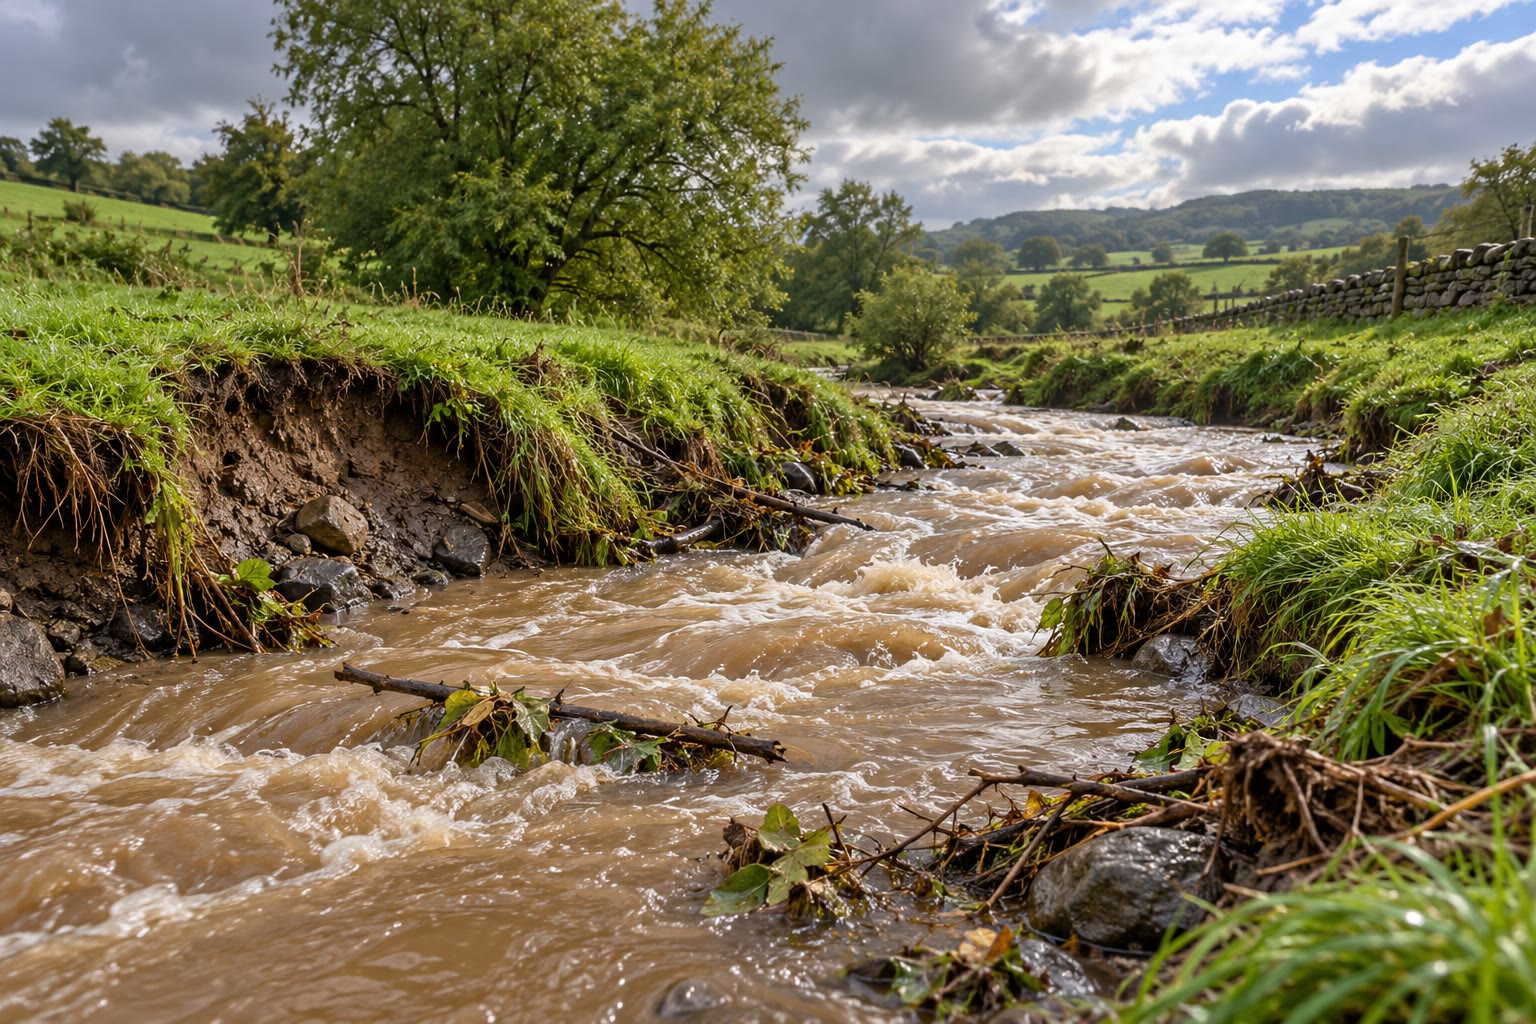
\includegraphics[width=0.5\linewidth]{images/book1/ai/g5-brown-stream.jpg}

{\small جدول في الصباح التالي لعاصفة: الماء بني من \omterm{def:g3:stones-pebbles-sand:sand}{الوحل} \omterm{def:g3:stones-pebbles-sand:sand}{والرمل}
اللذين يحملهما.}
\end{omfigure}

\begin{recall}
\omterm{def:g3:stones-pebbles-sand:rock}{الصخر} هو المادة الصلبة للأرض؛ وإذا تكسّر أعطى حجارة، \omterm{def:g3:stones-pebbles-sand:pebble}{وحصى} دوّرها الماء،
\omterm{def:g3:stones-pebbles-sand:sand}{ورملًا} نرى حباته واحدة واحدة، ووحلًا حباته أصغر من أن تُرى
(\cref{ch:g3:stones-pebbles-sand}). \omterm{def:g1:landscapes-around-us:water}{والنهر} يجري دائمًا في مجرى طويل، من
الأرض المرتفعة نزولًا إلى \omterm{def:g1:landscapes-around-us:water}{بحيرة} أو إلى \omterm{def:g2:water-on-earth:ocean}{البحر}
(\cref{ch:g1:landscapes-around-us}). \omterm{def:g4:clouds-rain-snow:precipitation}{والمطر} الذي يسقط على اليابسة يجري إلى
الجداول \omterm{def:g1:landscapes-around-us:water}{والأنهار}، وهي تعيد الماء إلى \omterm{def:g2:water-on-earth:ocean}{البحر}
(\cref{ch:g2:water-on-earth}).
\end{recall}

\section{الصخر يتفتت في مكانه}

حتى أصلب \omterm{def:g3:stones-pebbles-sand:rock}{الصخور} لا يدوم إلى الأبد. فحيث يكون مكشوفًا، تحت الشمس \omterm{def:g4:clouds-rain-snow:precipitation}{والمطر}
والصقيع، يتشقق ببطء ويتفتت.

\begin{definition}[التجوية]\label{def:g5:water-shapes-the-land:weathering}
\emph{التجوية}\index{تجوية} هي التفتت البطيء \omterm{def:g3:stones-pebbles-sand:rock}{للصخر} في مكانه، بفعل الصقيع،
والماء، وجذور النباتات، والحر والبرد. فيتكسر \omterm{def:g3:stones-pebbles-sand:rock}{الصخر} قطعًا، لكن القطع تبقى في
مكانها.
\end{definition}

الصقيع من أقوى أدوات \omterm{def:g5:water-shapes-the-land:weathering}{التجوية}. فماء \omterm{def:g4:clouds-rain-snow:precipitation}{المطر} يتسرب إلى شق رفيع في \omterm{def:g3:stones-pebbles-sand:rock}{الصخر}. وفي
ليلة باردة يتجمد، والماء حين يتجمد يشغل حيزًا أكبر قليلًا: فيضغط الجليد على
جانبي الشق ويوسعه قليلًا جدًا. وفي اليوم التالي يذوب الجليد، فيتسرب مزيد من
الماء، ثم يتجمد من جديد في الليلة التالية. وبعد شتاءات كثيرة، تنفصل قطعة من
\omterm{def:g3:stones-pebbles-sand:rock}{الصخر}.

\begin{omfigure}
\begin{tikzpicture}[x=1cm, y=1cm, font=\scriptsize]
  \foreach \i/\t in {0/{\foreignlanguage{arabic}{1. يتسرب ماء المطر}\\إلى شق},
                     4.3/{\foreignlanguage{arabic}{2. في الليل يتجمد}\\فيوسّع الجليد\\الشق},
                     8.6/{\foreignlanguage{arabic}{3. بعد شتاءات كثيرة}\\تنفصل قطعة}} {
    \begin{scope}[xshift=\i cm]
      \fill[gray!35] (0,0) rectangle (3.4,2.6);
      \draw[gray!60!black] (0,2.6) -- (3.4,2.6);
      \node[align=center, anchor=north] at (1.7,-0.15) {\t};
    \end{scope}
  }
  % panel 1: thin crack with water
  \fill[white] (1.55,2.6) -- (1.75,0.9) -- (1.85,2.6) -- cycle;
  \fill[blue!45] (1.6,2.2) -- (1.75,0.9) -- (1.83,2.2) -- cycle;
  \draw[gray!60!black] (1.55,2.6) -- (1.75,0.9) -- (1.85,2.6);
  \foreach \x in {1.3,1.7,2.1} \draw[blue!60, ->] (\x,3.3) -- (\x+0.05,2.8);
  \node[blue!60!black] at (0.6,3.1) {مطر};
  % panel 2: wider crack with ice
  \begin{scope}[xshift=4.3cm]
    \fill[white] (1.45,2.6) -- (1.75,0.75) -- (1.98,2.6) -- cycle;
    \fill[cyan!15] (1.5,2.3) -- (1.75,0.75) -- (1.94,2.3) -- cycle;
    \draw[cyan!50!black] (1.5,2.3) -- (1.75,0.75) -- (1.94,2.3) -- cycle;
    \draw[gray!60!black] (1.45,2.6) -- (1.75,0.75) -- (1.98,2.6);
    \draw[red!70!black, thick, <-] (1.05,1.9) -- (1.5,1.9);
    \draw[red!70!black, thick, ->] (1.98,1.9) -- (2.45,1.9);
    \node[cyan!40!black] at (1.72,3.0) {جليد};
  \end{scope}
  % panel 3: broken block
  \begin{scope}[xshift=8.6cm]
    \fill[white] (1.35,2.6) -- (1.75,0.6) -- (3.4,0.6) -- (3.4,2.6) -- cycle;
    \draw[gray!60!black] (1.35,2.6) -- (1.75,0.6) -- (3.4,0.6);
    \fill[gray!35, draw=gray!60!black, rotate around={-25:(2.9,0.3)}]
      (2.3,0.3) -- (2.4,1.4) -- (3.5,1.35) -- (3.4,0.3) -- cycle;
    \draw[gray!60!black, ->] (2.6,2.2) to[bend left=20] (3.0,1.5);
  \end{scope}
\end{tikzpicture}

{\small الصقيع يكسر \omterm{def:g3:stones-pebbles-sand:rock}{الصخر}. ففي كل ليلة صقيع، يضغط الجليد في الشق قليلًا؛ وبعد
شتاءات كثيرة، يصير الشق عريضًا بما يكفي لتنفصل
قطعة.}
\end{omfigure}

تحت جرف من \omterm{def:g3:stones-pebbles-sand:rock}{الصخر} العاري عاليًا في \omterm{def:g1:landscapes-around-us:landform}{الجبال}، تنزلق القطع التي كسرها الصقيع
وتتدحرج، فتتراكم في منحدر من الحجارة الحادة. وهي ليست مستديرة: فلم يدحرجها
الماء بعد.

\begin{omfigure}
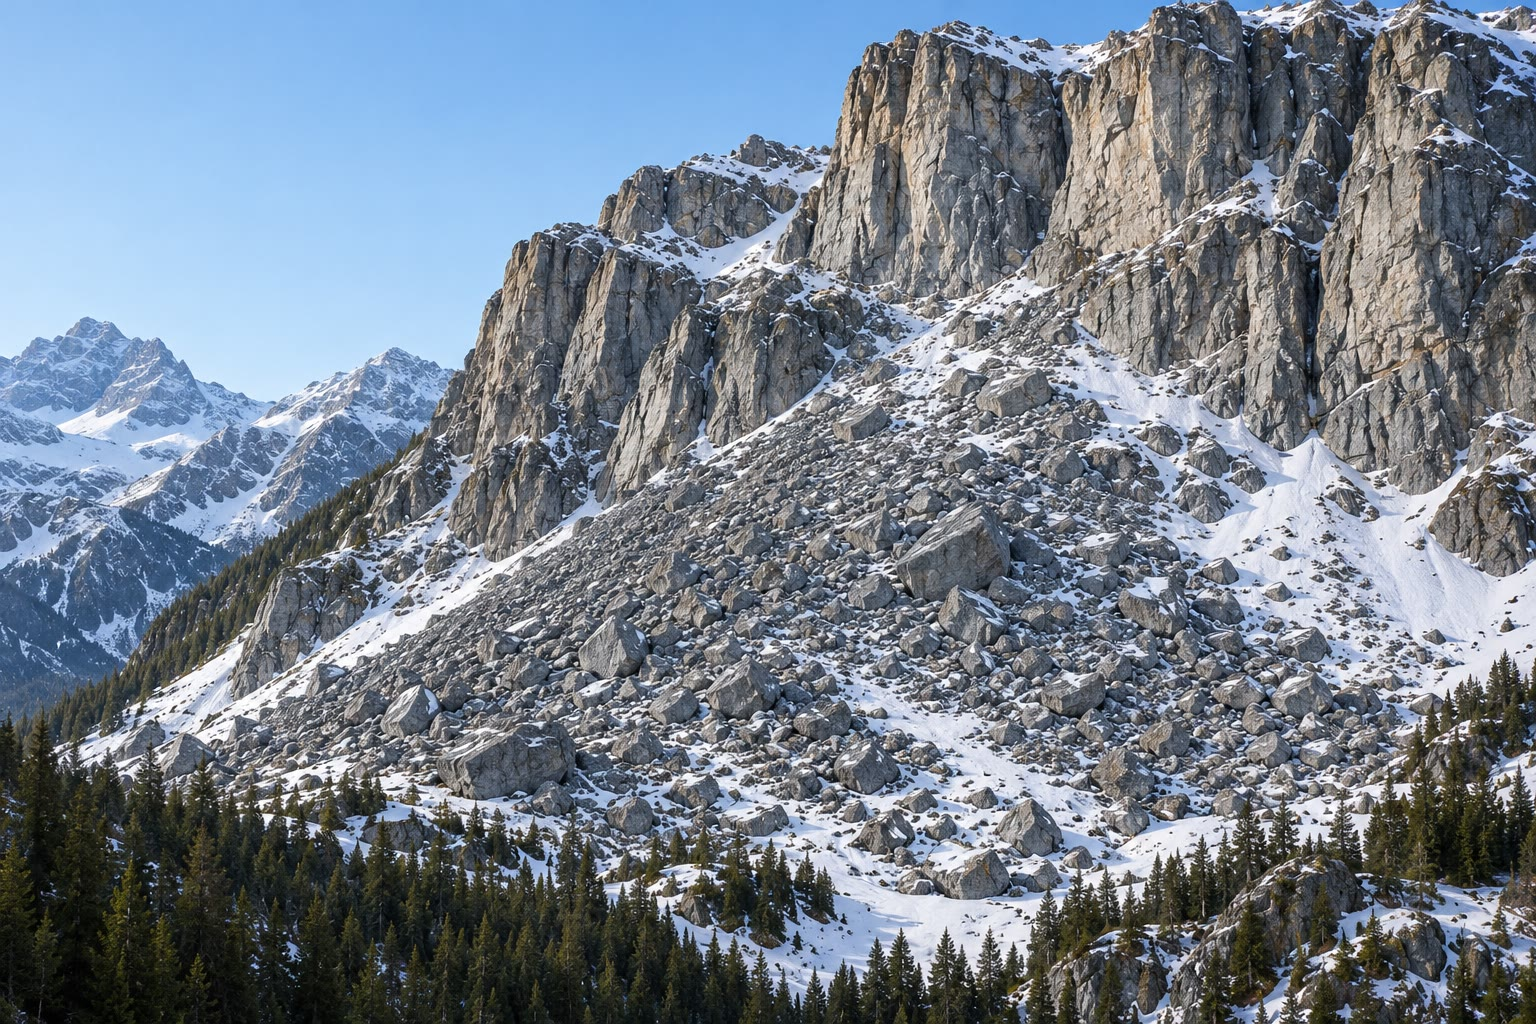
\includegraphics[width=0.5\linewidth]{images/book1/ai/g5-frost-scree.jpg}

{\small تحت جرف جبلي، منحدر من الحجارة الحادة الحواف كسرها الصقيع، كما يُرى
من الجهة الأخرى \omterm{def:g1:landscapes-around-us:landform}{للوادي}.}
\end{omfigure}

والنباتات تساعد أيضًا. فجذر الشجرة ينسلّ في شق، وحين يغلظ سنة بعد سنة، يشق
\omterm{def:g3:stones-pebbles-sand:rock}{الصخر} كإسفين بطيء. وماء \omterm{def:g4:clouds-rain-snow:precipitation}{المطر} نفسه يليّن بعض \omterm{def:g3:stones-pebbles-sand:rock}{الصخور} ببطء ويحولها إلى طين
\omterm{def:g3:stones-pebbles-sand:sand}{ورمل}: وهكذا تحصل التربة على حباتها
المعدنية.

\section{الماء يحمل القطع بعيدًا}

بعد أن يتكسر \omterm{def:g3:stones-pebbles-sand:rock}{الصخر}، تستطيع القطع أن تتحرك. لكن لا بد من شيء يحملها.

\begin{definition}[التعرية]\label{def:g5:water-shapes-the-land:erosion}
\emph{التعرية}\index{تعرية} هي بري اليابسة وحمل قطع \omterm{def:g3:stones-pebbles-sand:rock}{الصخر} بعيدًا، بفعل الماء
الجاري قبل كل شيء، وأيضًا بفعل الريح والجليد وأمواج
\omterm{def:g2:water-on-earth:ocean}{البحر}.
\end{definition}

الماء الجاري يقوم بمعظم العمل. \omterm{def:g4:clouds-rain-snow:precipitation}{فالمطر} يجرف التربة والحبات على المنحدرات إلى
الجداول؛ والجداول تنتزع المزيد من ضفافها هي، كما فعل جدول توم ولينا بعد
العاصفة. وكلما جرى الماء أسرع، استطاع أن يحمل أكثر، وأن يحرك قطعًا أكبر:
فالجدول الهادئ لا يحمل إلا \omterm{def:g3:stones-pebbles-sand:sand}{الوحل} الناعم؛ أما الجدول في فيضانه فيدحرج \omterm{def:g3:stones-pebbles-sand:pebble}{الحصى} بل
الجلاميد في قاعه.

وفي طريقها تصطدم الحجارة بعضها ببعض وبالقاع. فتنكسر زواياها، فتصير \omterm{def:g3:stones-pebbles-sand:pebble}{حصى}
مستديرًا، ثم حبات أصغر فأصغر: \omterm{def:g3:stones-pebbles-sand:sand}{رملًا}
ووحلًا.

والريح تقوم بالعمل نفسه في الأماكن الجافة، حيث لا شيء يمسك \omterm{def:g3:stones-pebbles-sand:sand}{الرمل}: فتذروه
كثبانًا. والجليد، في \omterm{def:g1:landscapes-around-us:landform}{الجبال} وقرب \omterm{def:g3:continents-and-oceans:poles}{القطبين}، يجر الحجارة تحت ثقله الهائل. وعلى
\omterm{def:g1:landscapes-around-us:water}{الساحل}، تضرب الأمواج الجروف وتدحرج \omterm{def:g3:stones-pebbles-sand:pebble}{حصى} الشاطئ ذهابًا
وإيابًا.

\begin{remark}[كم؟]\label{rem:g5:water-shapes-the-land:how-much}
\omterm{def:g1:landscapes-around-us:water}{أنهار} العالم كلها معًا تحمل إلى \omterm{def:g2:water-on-earth:ocean}{البحر} أكثر من 12 مليار طن من \omterm{def:g3:stones-pebbles-sand:sand}{الوحل} \omterm{def:g3:stones-pebbles-sand:sand}{والرمل}
كل سنة. أي نحو مليار طن كل
شهر.
% ledger: syvitski:modern-flux
\end{remark}

\section{الماء يضع القطع}

لا يستطيع \omterm{def:g1:landscapes-around-us:water}{النهر} أن يحمل حمولته إلى الأبد. فحيث يتباطأ، لا تبقى له القوة
ليحرك أكبر حباته، فتستقر في قاعه.

\begin{definition}[الترسيب]\label{def:g5:water-shapes-the-land:deposition}
\emph{الترسيب}\index{ترسيب} هو وضع قطع \omterm{def:g3:stones-pebbles-sand:rock}{الصخر} التي حملها الماء أو الريح أو
الجليد، حيث تتباطأ وتتوقف.
\end{definition}

أثقل القطع تستقر أولًا: \omterm{def:g3:stones-pebbles-sand:pebble}{فالحصى} يسقط حيث يضعف التيار قليلًا، \omterm{def:g3:stones-pebbles-sand:sand}{والرمل} حيث
يتباطأ أكثر، \omterm{def:g3:stones-pebbles-sand:sand}{والوحل} الناعم لا يسقط إلا حيث يكاد الماء يسكن، في \omterm{def:g1:landscapes-around-us:water}{بحيرة} أو في
\omterm{def:g2:water-on-earth:ocean}{البحر}. ولهذا يكون قاع \omterm{def:g1:landscapes-around-us:water}{النهر} حصويًا في \omterm{def:g1:landscapes-around-us:landform}{الجبال}، ورمليًا أو موحلًا قرب
\omterm{def:g2:water-on-earth:ocean}{البحر}.

\omterm{def:g5:water-shapes-the-land:weathering}{التجوية} \omterm{def:g5:water-shapes-the-land:erosion}{والتعرية} \omterm{def:g5:water-shapes-the-land:deposition}{والترسيب} ثلاث مراحل من رحلة واحدة طويلة: يتفتت \omterm{def:g3:stones-pebbles-sand:rock}{الصخر} في
مكانه، وتُحمل قطعه بعيدًا، ثم توضع في مكان آخر. وببطء، ينقل الماء \omterm{def:g1:landscapes-around-us:landform}{الجبال}،
حبة بعد حبة، نزولًا إلى \omterm{def:g1:landscapes-around-us:landform}{السهول} وإلى
\omterm{def:g2:water-on-earth:ocean}{البحر}.

\begin{method}[تسمية ما يفعله الماء]\label{met:g5:water-shapes-the-land:naming}
لتسمّي ما يحدث \omterm{def:g3:stones-pebbles-sand:rock}{للصخر} في صورة أو في قصة، اطرح ثلاثة
أسئلة:
\begin{enumerate}
  \item هل يتكسر \omterm{def:g3:stones-pebbles-sand:rock}{الصخر}، لكن القطع تبقى حيث هي؟
        تلك \emph{\omterm{def:g5:water-shapes-the-land:weathering}{تجوية}}.
  \item هل تُبرى القطع وتُحمل بعيدًا؟ تلك
        \emph{\omterm{def:g5:water-shapes-the-land:erosion}{تعرية}}.
  \item هل تستقر القطع وتتراكم؟ ذلك
        \emph{\omterm{def:g5:water-shapes-the-land:deposition}{ترسيب}}.
\end{enumerate}
\end{method}

\begin{example}[الجدول بعد العاصفة]\label{ex:g5:water-shapes-the-land:stream}
ماء جدول توم ولينا البني يحمل وحلًا انتزعه من ضفتيه:
تلك \omterm{def:g5:water-shapes-the-land:erosion}{تعرية}. وبعد أسبوع، يعود الجدول صافيًا، وتغطي طبقة رقيقة
من \omterm{def:g3:stones-pebbles-sand:sand}{الوحل} قاع البركة الهادئة في طرف الساحة:
ذلك \omterm{def:g5:water-shapes-the-land:deposition}{ترسيب}.
\end{example}

\section{النهر من منبعه إلى مصبه}

لكل \omterm{def:g1:landscapes-around-us:water}{نهر} بداية ونهاية.

\begin{definition}[المنبع والمصب والرافد]\label{def:g5:water-shapes-the-land:source-mouth}
\emph{منبع}\index{منبع (نهر)} \omterm{def:g1:landscapes-around-us:water}{النهر} هو المكان الذي يبدأ منه: عين ماء، أو
\omterm{def:g1:landscapes-around-us:water}{نهر} جليدي يذوب، أو أرض عالية رطبة تبدأ فيها جداول صغيرة كثيرة جدًا.
و\emph{مصبه}\index{مصب (نهر)} هو المكان الذي ينتهي فيه، فيصب في \omterm{def:g2:water-on-earth:ocean}{البحر} أو في
\omterm{def:g1:landscapes-around-us:water}{بحيرة} أو في \omterm{def:g1:landscapes-around-us:water}{نهر} أكبر. و\emph{الرافد}\index{رافد} \omterm{def:g1:landscapes-around-us:water}{نهر} أصغر يصب في
\omterm{def:g1:landscapes-around-us:water}{نهر} أكبر.
\end{definition}

وعلى طول طريقه، يتغير \omterm{def:g1:landscapes-around-us:water}{النهر}. فنقسم طوله ثلاثة أجزاء: مجراه الأعلى، ومجراه
الأوسط، ومجراه الأدنى.

\begin{omfigure}
\begin{tikzpicture}[x=1.15cm, y=1cm, font=\scriptsize]
  % ground
  \fill[brown!25] (0,-0.6) -- plot[domain=0:11, samples=60]
    (\x,{4.6*exp(-\x/2.4)}) -- (11,-0.6) -- cycle;
  % sea
  \fill[blue!20] (11,-0.6) rectangle (12.6,0.02);
  \draw[blue!70!black, line width=1.3pt] plot[domain=0.15:11, samples=60]
    (\x,{4.6*exp(-\x/2.4)});
  \draw[gray] (11,0.02) -- (12.6,0.02);
  \node[blue!50!black] at (11.9,-0.3) {البحر};
  % course limits
  \foreach \x in {2.6,6.6} \draw[gray, dashed] (\x,-0.6) -- (\x,5.4);
  \node[align=center, anchor=north] at (1.3,6.3) {\textbf{المجرى الأعلى}\\شديد الانحدار وسريع\\\foreignlanguage{arabic}{وادٍ على شكل حرف \babelsublr{V}}};
  \node[align=center, anchor=north] at (4.6,6.3) {\textbf{المجرى الأوسط}\\انحدار ألطف\\منعطفات};
  \node[align=center, anchor=north] at (8.8,6.3) {\textbf{المجرى الأدنى}\\شبه مستوٍ وبطيء\\سهل فيضي واسع};
  % source and mouth
  \fill[blue!70!black] (0.15,{4.6*exp(-0.15/2.4)}) circle (2pt);
  \node[anchor=east] at (0.05,3.7) {المنبع};
  \draw[->] (0.05,3.75) -- (0.12,4.15);
  \node[anchor=south] at (11.4,0.75) {المصب};
  \draw[->] (11.4,0.75) -- (11.05,0.15);
  % grain sizes
  \node[anchor=north, align=center, text=brown!50!black] at (1.3,-0.7) {جلاميد وحصى};
  \node[anchor=north, align=center, text=brown!50!black] at (4.6,-0.7) {حصى ورمل};
  \node[anchor=north, align=center, text=brown!50!black] at (8.8,-0.7) {رمل ووحل};
  \node[anchor=north, align=center, text=brown!50!black] at (11.8,-0.7) {وحل};
\end{tikzpicture}

{\small المقطع الطولي \omterm{def:g1:landscapes-around-us:water}{لنهر}، من \omterm{def:g5:water-shapes-the-land:source-mouth}{منبعه} إلى \omterm{def:g5:water-shapes-the-land:source-mouth}{مصبه} (الارتفاعات مضخّمة كثيرًا).
وفي الأسفل: ما يوجد في قاعه.}
\end{omfigure}

في \emph{مجراه الأعلى}، في \omterm{def:g1:landscapes-around-us:landform}{الجبال}، يكون \omterm{def:g1:landscapes-around-us:water}{النهر} فتيًا شديد الانحدار. فماؤه
يندفع نزولًا، ويدحرج الجلاميد في قاعه، ويحفر نحو الأسفل في \omterm{def:g3:stones-pebbles-sand:rock}{الصخر}. فيحفر \omterm{def:g1:landscapes-around-us:landform}{واديًا}
ضيقًا جانباه شديدا الانحدار، على شكل
الحرف V.

وفي \emph{مجراه الأوسط}، يكون الانحدار ألطف. فيتمايل \omterm{def:g1:landscapes-around-us:water}{النهر} من جانب إلى جانب
في حلقات كبيرة.

\begin{definition}[المنعطف النهري]\label{def:g5:water-shapes-the-land:meander}
\emph{المنعطف النهري}\index{منعطف نهري} حلقة من \omterm{def:g1:landscapes-around-us:water}{نهر} تتلوى عبر قاع واد
مستوٍ.
\end{definition}

\omterm{def:g5:water-shapes-the-land:meander}{المنعطف} لا يبقى ساكنًا: إنه يتحرك. ففي الجهة الخارجية لكل انعطاف، يجري الماء
سريعًا عميقًا: فيأكل الضفة، فتصير جرفًا صغيرًا. وفي الجهة الداخلية للانعطاف،
يجري الماء ببطء: فيضع \omterm{def:g3:stones-pebbles-sand:sand}{رملًا} \omterm{def:g3:stones-pebbles-sand:pebble}{وحصباء}، يبنيان شاطئًا لطيف الانحدار. وسنة بعد
سنة، تتراجع الضفة الخارجية ويكبر الشاطئ الداخلي، فتتسع الحلقة أكثر
فأكثر.

\begin{omfigure}
\begin{tikzpicture}[x=1cm, y=1cm, font=\scriptsize]
  % ---- map view ----
  \fill[green!12] (-0.4,-2.5) rectangle (6.4,2.5);
  % sand on the inner banks (drawn first, the river covers its edge)
  \foreach \c/\s in {1/1, 3/-1, 5/1}
    \fill[yellow!50!orange!45] (\c-0.6,\s*0.5) .. controls (\c,\s*1.5) ..
      (\c+0.6,\s*0.5) .. controls (\c,\s*0.75) .. cycle;
  % the river
  \draw[blue!35, line width=11pt] plot[domain=-0.3:6.3, samples=90]
    (\x,{1.25*sin(\x*90)});
  \draw[blue!70!black, ->, thick] plot[domain=1.6:2.4, samples=10]
    (\x,{1.25*sin(\x*90)});
  \draw[blue!70!black, ->, thick] plot[domain=3.6:4.4, samples=10]
    (\x,{1.25*sin(\x*90)});
  % erosion on the outer banks
  \foreach \c/\s in {1/1, 3/-1, 5/1}
    \foreach \d in {-0.3,0,0.3}
      \draw[red!70!black, thick, ->] (\c+\d,{\s*(1.25*cos(\d*90)+0.22)})
        -- (\c+\d,{\s*(1.25*cos(\d*90)+0.6)});
  \node[red!70!black] at (1,2.2) {\foreignlanguage{arabic}{تعرية: الضفة الخارجية}};
  \node[red!70!black] at (3,-2.2) {\foreignlanguage{arabic}{تعرية: الضفة الخارجية}};
  \node[orange!40!black, align=center] (d1) at (1,-0.55) {ترسيب\\الضفة الداخلية};
  \node[orange!40!black, align=center] (d2) at (3,0.55) {ترسيب\\الضفة الداخلية};
  \draw[orange!40!black] (d1.north) -- (1,0.7);
  \draw[orange!40!black] (d2.south) -- (3,-0.7);
  \draw[gray!50!black, dashed] (5,0.15) -- (5,2.3);
  \node[gray!50!black, anchor=north] at (5,0.15) {مقطع};
  \node[gray!50!black, anchor=east] at (4.95,0.35) {A};
  \node[gray!50!black, anchor=east] at (4.95,2.15) {B};
  \node[anchor=west] at (6.5,0) {منظر من الأعلى};
  % ---- cut ----
  \begin{scope}[yshift=-4.1cm, xscale=0.77]
    \fill[brown!25] (-0.4,-1.3) -- (-0.4,0.9) -- (1,0.9) -- (3.6,-0.8)
      .. controls (4.4,-1.05) .. (4.9,-0.9) -- (5.1,0.9) -- (8.4,0.9)
      -- (8.4,-1.3) -- cycle;
    \fill[blue!25] (1.75,0.4) -- (3.6,-0.8) .. controls (4.4,-1.05) .. (4.9,-0.9)
      -- (5.04,0.4) -- cycle;
    \fill[yellow!50!orange!40] (1,0.9) -- (3.6,-0.8) -- (2.6,-0.8) -- cycle;
    \draw[gray!60!black] (-0.4,0.9) -- (1,0.9) -- (3.6,-0.8)
      .. controls (4.4,-1.05) .. (4.9,-0.9) -- (5.1,0.9) -- (8.4,0.9);
    \draw[blue!60!black] (1.75,0.4) -- (5.04,0.4);
    \node[orange!40!black, align=center] at (0.9,-0.4) {الضفة الداخلية\\ماء بطيء\\شاطئ رملي};
    \node[red!70!black, align=center, anchor=west] at (5.3,-0.3) {الضفة الخارجية\\ماء سريع عميق\\جرف صغير};
    \draw[red!70!black, thick, ->] (4.6,-0.2) -- (5.0,-0.2);
    \node[gray!50!black, anchor=south] at (-0.2,0.9) {A};
    \node[gray!50!black, anchor=south] at (8.2,0.9) {B};
    \node[anchor=west] at (8.45,0) {\foreignlanguage{arabic}{المقطع \babelsublr{A--B}}};
  \end{scope}
\end{tikzpicture}

{\small \omterm{def:g5:water-shapes-the-land:meander}{منعطف} يُرى من الأعلى، ومقطوعًا على طول الخط المتقطع A--B. فالماء
يبري الضفة الخارجية لكل انعطاف ويضع \omterm{def:g3:stones-pebbles-sand:sand}{الرمل} على الضفة الداخلية: فتتحرك الحلقة
ببطء.}
\end{omfigure}

وأحيانًا تقترب حلقتان إلى حد أن \omterm{def:g1:landscapes-around-us:water}{النهر}، أثناء \omterm{def:g5:water-shapes-the-land:flood}{فيضان}، يخترق عنق الأرض الضيق
بينهما ويسلك الطريق المختصر. فتُترك الحلقة القديمة وراءه بحيرةً
مقوسة.

\begin{omfigure}
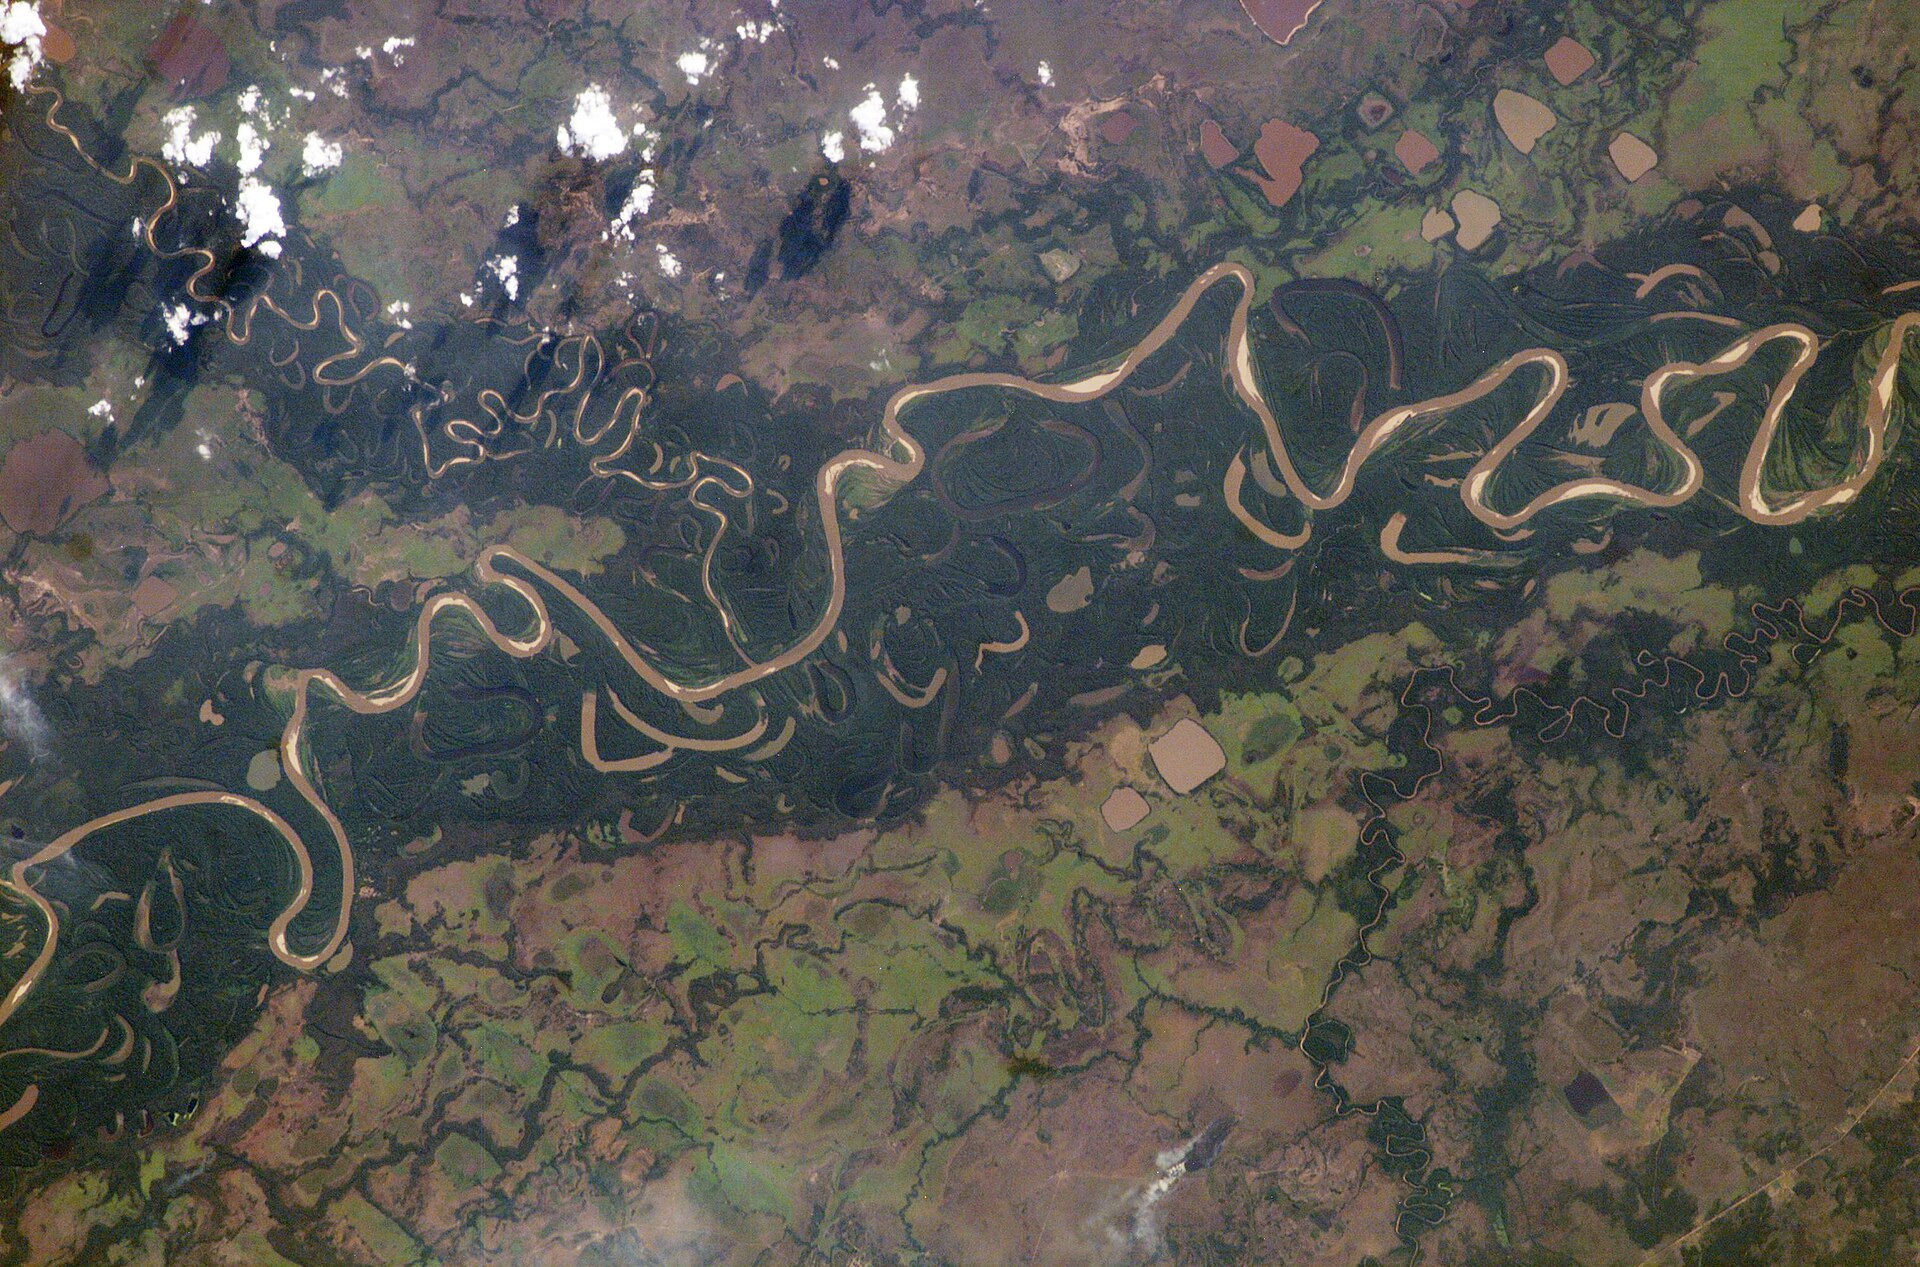
\includegraphics[width=0.52\linewidth]{images/book1/g5-mamore-meanders.jpg}

{\small \omterm{def:g1:landscapes-around-us:water}{نهر} ماموري، في الأراضي المنخفضة في بوليفيا بأمريكا الجنوبية، كما يُرى
من محطة الفضاء الدولية. يتلوى \omterm{def:g1:landscapes-around-us:water}{النهر} البني في \omterm{def:g5:water-shapes-the-land:meander}{منعطفات}
عبر الغابة. الصورة: NASA (ملك عام).}\label{fig:g5:water-shapes-the-land:mamore}
% ledger: nasa:mamore-meanders
\end{omfigure}

وفي \emph{مجراه الأدنى}، تكون الأرض شبه مستوية. فيجري \omterm{def:g1:landscapes-around-us:water}{النهر} ببطء عبر قاع واد
عريض مستوٍ، صنعه من \omterm{def:g3:stones-pebbles-sand:sand}{الوحل} \omterm{def:g3:stones-pebbles-sand:sand}{والرمل} اللذين وضعهما هو نفسه على مدى زمن طويل
جدًا.

\begin{omfigure}
\begin{tikzpicture}[x=1cm, y=1cm, font=\scriptsize]
  % V-shaped valley
  \fill[gray!30] (0,0) -- (0,2.6) -- (0.5,2.6) -- (2.3,0.45) -- (2.7,0.45)
    -- (4.5,2.6) -- (5,2.6) -- (5,0) -- cycle;
  \fill[blue!35] (2.3,0.45) -- (2.4,0.25) -- (2.6,0.25) -- (2.7,0.45) -- cycle;
  \draw[gray!60!black] (0,2.6) -- (0.5,2.6) -- (2.3,0.45) -- (2.4,0.25)
    -- (2.6,0.25) -- (2.7,0.45) -- (4.5,2.6) -- (5,2.6);
  \draw[red!70!black, thick, ->] (2.5,1.9) -- (2.5,0.6);
  \node[red!70!black, anchor=south] at (2.5,1.9) {يحفر نحو الأسفل};
  \node[align=center, anchor=north] at (2.5,-0.1) {المجرى الأعلى\\\foreignlanguage{arabic}{وادٍ ضيق على شكل حرف \babelsublr{V}}};
  % floodplain
  \begin{scope}[xshift=6cm]
    \fill[gray!30] (0,0) -- (0,2.6) -- (0.6,2.6) -- (1.3,0.9) -- (5.7,0.9)
      -- (6.4,2.6) -- (7,2.6) -- (7,0) -- cycle;
    \fill[brown!25] (1.3,0.9) -- (1.55,0.3) -- (5.45,0.3) -- (5.7,0.9) -- cycle;
    \fill[blue!35] (3.1,0.9) -- (3.25,0.62) -- (3.85,0.62) -- (4,0.9) -- cycle;
    \draw[gray!60!black] (0,2.6) -- (0.6,2.6) -- (1.3,0.9) -- (3.1,0.9)
      -- (3.25,0.62) -- (3.85,0.62) -- (4,0.9) -- (5.7,0.9) -- (6.4,2.6) -- (7,2.6);
    \draw[blue!60!black, dashed] (1.22,1.1) -- (5.78,1.1);
    \node[blue!50!black, anchor=south] at (2.0,1.12) {في الفيضان};
    \node[brown!50!black] at (2.2,0.55) {وحل ورمل};
    \draw[<->] (1.3,1.75) -- (5.7,1.75);
    \node[anchor=south] at (3.5,1.75) {السهل الفيضي};
    \node[align=center, anchor=north] at (3.5,-0.1) {المجرى الأدنى\\قاع واد عريض مستوٍ};
  \end{scope}
\end{tikzpicture}

{\small \omterm{def:g1:landscapes-around-us:landform}{الوادي} مقطوعًا عرضيًا، في \omterm{def:g1:landscapes-around-us:landform}{الجبال} وقرب \omterm{def:g2:water-on-earth:ocean}{البحر} (ليسا بمقياس الرسم
نفسه). وفي \omterm{def:g5:water-shapes-the-land:flood}{الفيضان}، ينتشر \omterm{def:g1:landscapes-around-us:water}{النهر} على \omterm{def:g5:water-shapes-the-land:flood}{سهله الفيضي} كله.}
\end{omfigure}

وأخيرًا يبلغ \omterm{def:g1:landscapes-around-us:water}{النهر} \omterm{def:g5:water-shapes-the-land:source-mouth}{مصبه}. وهناك يتباطأ الماء حتى يكاد يتوقف تمامًا، فيضع
\omterm{def:g1:landscapes-around-us:water}{النهر} آخر حمولته. وحيث تكون أمواج \omterm{def:g2:water-on-earth:ocean}{البحر} ومده وجزره أضعف من أن تحملها كلها
بعيدًا، يتراكم \omterm{def:g3:stones-pebbles-sand:sand}{الوحل} \omterm{def:g3:stones-pebbles-sand:sand}{والرمل}، وتنمو أرض جديدة داخل
\omterm{def:g2:water-on-earth:ocean}{البحر}.

\begin{definition}[الدلتا]\label{def:g5:water-shapes-the-land:delta}
\emph{الدلتا}\index{دلتا} أرض جديدة مستوية يبنيها \omterm{def:g1:landscapes-around-us:water}{النهر} عند \omterm{def:g5:water-shapes-the-land:source-mouth}{مصبه} من \omterm{def:g3:stones-pebbles-sand:sand}{الوحل}
\omterm{def:g3:stones-pebbles-sand:sand}{والرمل} اللذين يضعهما. وينقسم \omterm{def:g1:landscapes-around-us:water}{النهر} فيها فروعًا عدة تنتشر عبرها، كثيرًا ما
تكون على شكل مروحة.
\end{definition}

والاسم مأخوذ من الحرف اليوناني $\Delta$ (\omterm{def:g5:water-shapes-the-land:delta}{دلتا})، وهو مثلث،
لأن \omterm{def:g5:water-shapes-the-land:delta}{دلتا} النيل، في مصر، لها هذا الشكل.

وبعض \omterm{def:g1:landscapes-around-us:water}{الأنهار} تنتهي دون \omterm{def:g5:water-shapes-the-land:delta}{دلتا}. فحيث تجرف الأمواج القوية والمد والجزر \omterm{def:g3:stones-pebbles-sand:sand}{الوحل}
بعيدًا، ينتهي \omterm{def:g1:landscapes-around-us:water}{النهر} في \omterm{def:g5:water-shapes-the-land:source-mouth}{مصب} عريض على شكل قمع يدخله \omterm{def:g2:water-on-earth:ocean}{البحر} ويخرج منه مع المد
والجزر: \emph{\omterm{def:g5:water-shapes-the-land:source-mouth}{مصب} خليجي}.

\begin{omfigure}
\begin{minipage}[b]{0.55\linewidth}\centering
\begin{tikzpicture}[x=0.68cm, y=0.62cm, font=\scriptsize]
  \fill[blue!20] (-3.6,1.4) rectangle (3.6,3.6);
  \fill[green!15] (-3.6,-1.6) rectangle (3.6,1.4);
  % delta
  \fill[olive!35] (-2.6,1.4) .. controls (-2.2,2.4) and (-1,2.9)
    .. (0,3.0) .. controls (1,2.9) and (2.2,2.4) .. (2.6,1.4) -- cycle;
  \draw[gray!60!black] (-3.6,1.4) -- (-2.6,1.4) .. controls (-2.2,2.4) and
    (-1,2.9) .. (0,3.0) .. controls (1,2.9) and (2.2,2.4) .. (2.6,1.4) -- (3.6,1.4);
  \draw[gray!60!black, dashed] (-2.6,1.4) -- (2.6,1.4);
  % river and branches
  \draw[blue!60!black, line width=2pt] (0,-1.6) .. controls (0.3,-0.5) .. (0,0.9);
  \foreach \e in {-1.9,-0.9,0.2,1.2,2.0}
    \draw[blue!60!black, line width=1pt] (0,0.9) .. controls (\e*0.3,1.6) ..
      (\e,{2.95-0.3*\e*\e});
  % mud plume
  \fill[brown!30, opacity=0.5] (-1.3,3.05) .. controls (0,3.6) .. (1.3,3.0)
    .. controls (0,3.25) .. cycle;
  \node[align=center] at (-2.8,3.1) {البحر};
  \node[anchor=west, brown!50!black] at (1.35,3.25) {وحل};
  \node[anchor=west, align=left] at (3.7,2.4) {الدلتا\\أرض جديدة};
  \draw (3.7,2.4) -- (2.0,2.2);
  \node[anchor=west, align=left, gray!50!black] at (3.7,1.0) {الساحل\\القديم};
  \draw[gray!50!black] (3.7,1.0) -- (2.3,1.4);
  \node[anchor=west] at (0.35,-1.1) {النهر};
\end{tikzpicture}
\end{minipage}\hfill
\begin{minipage}[b]{0.3\linewidth}\centering
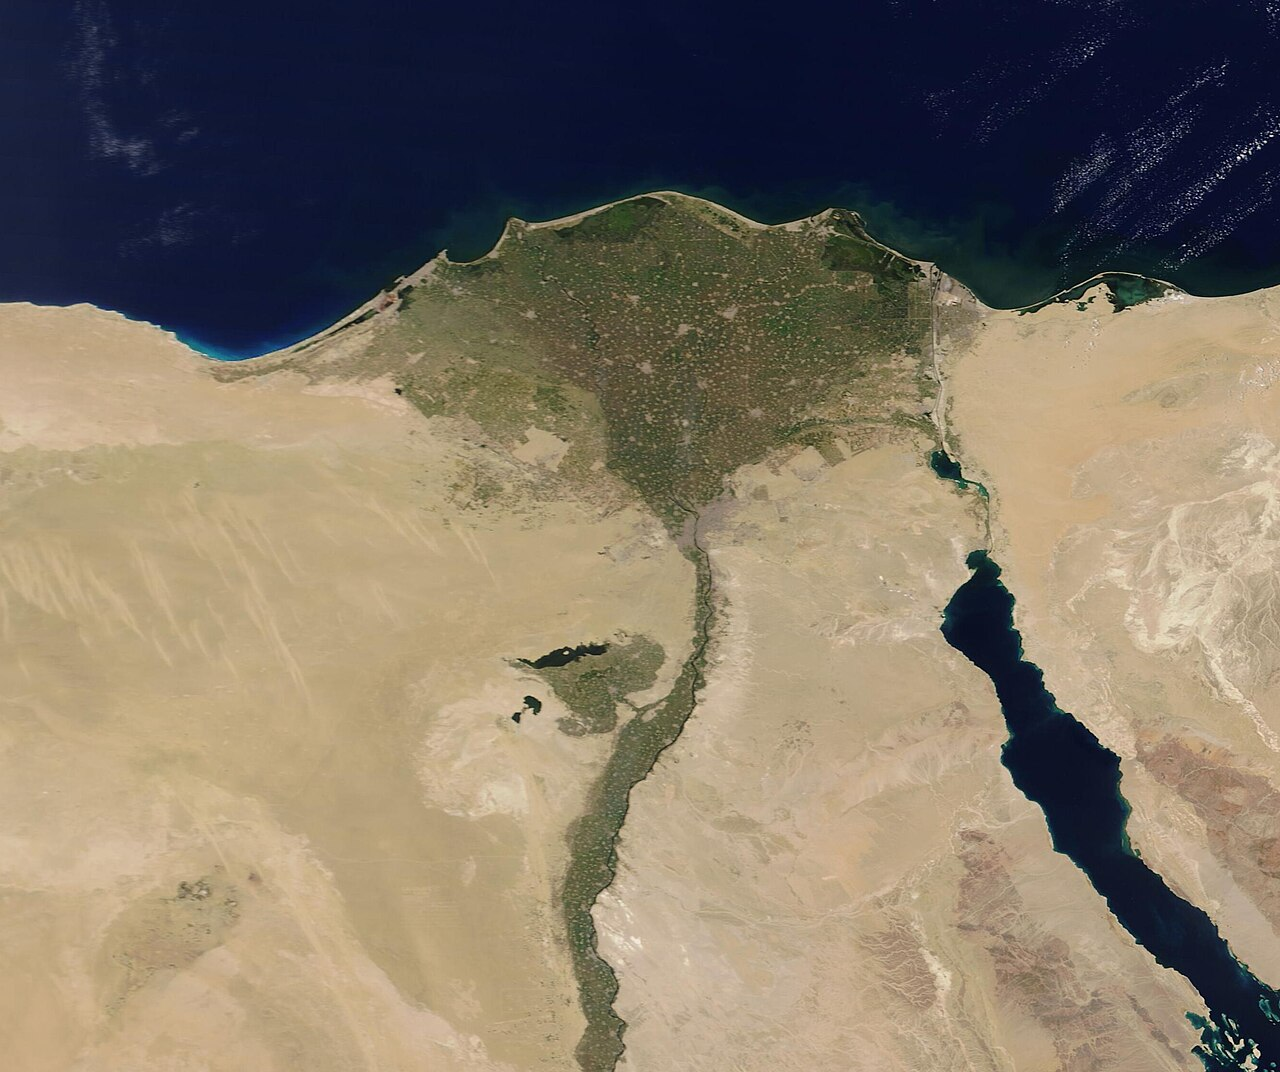
\includegraphics[width=\linewidth]{images/book1/g5-nile-delta-modis.jpg}
\end{minipage}

{\small إلى اليمين: \omterm{def:g5:water-shapes-the-land:delta}{دلتا} تُرى من الأعلى؛ \omterm{def:g3:stones-pebbles-sand:sand}{فالوحل} \omterm{def:g3:stones-pebbles-sand:sand}{والرمل} اللذان تضعهما
الفروع يبنيان أرضًا جديدة وراء \omterm{def:g1:landscapes-around-us:water}{الساحل} القديم. إلى اليسار: \omterm{def:g5:water-shapes-the-land:delta}{دلتا} النيل، في
مصر، من قمر صناعي (\omterm{def:g2:water-on-earth:ocean}{البحر} في الأعلى): مروحة خضراء من الحقول على \omterm{def:g3:stones-pebbles-sand:sand}{وحل}
\omterm{def:g1:landscapes-around-us:water}{النهر}، وسط الصحراء. الصورة: NASA (ملكية
عامة).}
% ledger: nasa:nile-delta-modis
\end{omfigure}

\section{الفيضانات}

بعد أيام طويلة من \omterm{def:g4:clouds-rain-snow:precipitation}{المطر}، أو حين يذوب \omterm{def:g4:clouds-rain-snow:precipitation}{الثلج} سريعًا في الربيع، يتلقى \omterm{def:g1:landscapes-around-us:water}{النهر}
من الماء أكثر مما يتسع له مجراه.

\begin{definition}[الفيضان والسهل الفيضي]\label{def:g5:water-shapes-the-land:flood}
يحدث \emph{الفيضان}\index{فيضان} حين يغطي الماء أرضًا تكون عادة جافة.
ويفيض \omterm{def:g1:landscapes-around-us:water}{النهر} حين يرتفع فوق ضفتيه وينتشر على الأرض المستوية على جانبيه.
وتلك الأرض المستوية، التي يغطيها \omterm{def:g1:landscapes-around-us:water}{النهر} من حين إلى آخر، هي
\emph{سهله الفيضي}\index{سهل فيضي}.
\end{definition}

\begin{omfigure}
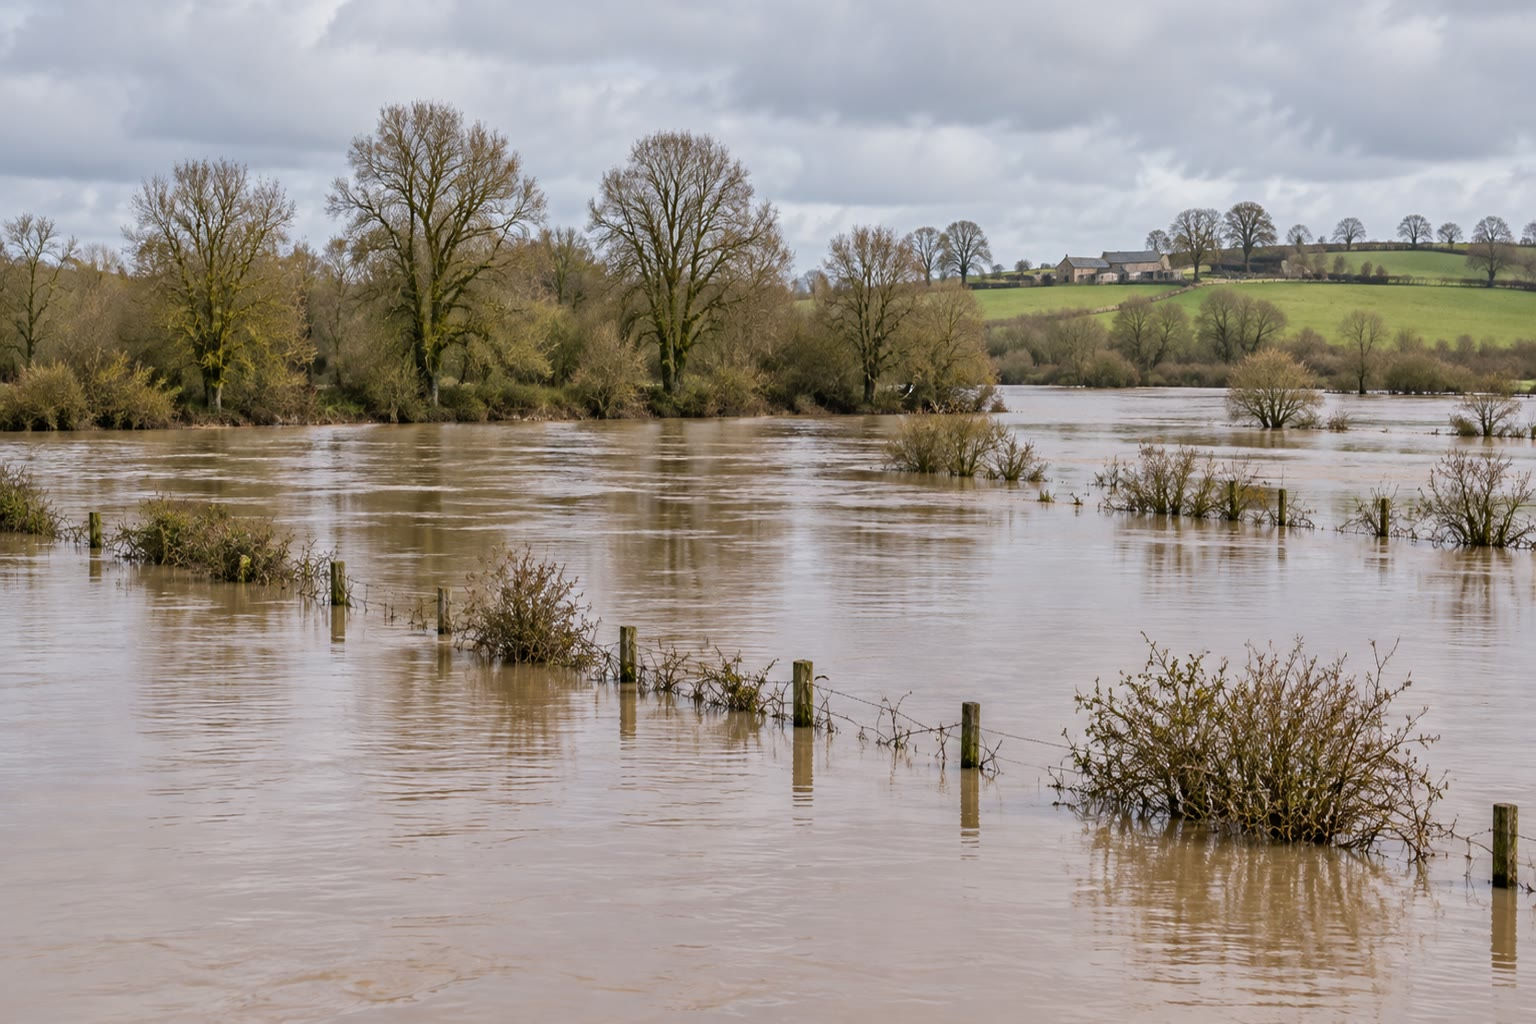
\includegraphics[width=0.5\linewidth]{images/book1/ai/g5-flooded-meadow.jpg}

{\small مرج تغمره مياه \omterm{def:g5:water-shapes-the-land:flood}{الفيضان} بعد أيام من \omterm{def:g4:clouds-rain-snow:precipitation}{المطر}. صف الأشجار يحدد الضفة
المعتادة \omterm{def:g1:landscapes-around-us:water}{للنهر}؛ والمزرعة تقوم على أرض أعلى.}
\end{omfigure}

\omterm{def:g1:landscapes-around-us:water}{النهر} الذي يفيض لا يفعل شيئًا غريبًا: إنه يفعل ما فعلته \omterm{def:g1:landscapes-around-us:water}{الأنهار} دائمًا.
\omterm{def:g5:water-shapes-the-land:flood}{فالسهل الفيضي} أرضه. بل إن \omterm{def:g1:landscapes-around-us:water}{النهر} هو الذي بناه: فكل \omterm{def:g5:water-shapes-the-land:flood}{فيضان} يترك طبقة رقيقة من
\omterm{def:g3:stones-pebbles-sand:sand}{الوحل} على الحقول، ولهذا تكون تربة \omterm{def:g1:landscapes-around-us:landform}{السهول} الفيضية خصبة جدًا. ومنذ زمن بعيد،
كان المزارعون في مصر ينتظرون \omterm{def:g5:water-shapes-the-land:flood}{فيضان} النيل السنوي، الذي كان يروي حقولهم
ويأتيهم \omterm{def:g3:stones-pebbles-sand:sand}{بوحل} جديد.

لكن \omterm{def:g5:water-shapes-the-land:flood}{الفيضان} خطر على الناس الذين يعيشون في \omterm{def:g5:water-shapes-the-land:flood}{السهل الفيضي}. فالبيوت المبنية فيه
قد تمتلئ بالماء، ومياه \omterm{def:g5:water-shapes-the-land:flood}{الفيضان} السريعة قد تجرف السيارات والناس. والمدينة
الحكيمة تبني على أرض أعلى وتترك \omterm{def:g5:water-shapes-the-land:flood}{السهل الفيضي} للحقول والمروج والحدائق. وفي
\cref{ch:g5:natural-hazards}
سنرى كيف يستعد الناس \omterm{def:g5:water-shapes-the-land:flood}{للفيضانات} ويبقون في أمان.

\begin{safety}
لا تمشِ أبدًا في مياه \omterm{def:g5:water-shapes-the-land:flood}{الفيضان}، ولا تركب فيها دراجة، ولا تلعب فيها، ولا تقترب
أبدًا من \omterm{def:g1:landscapes-around-us:water}{نهر} في فيضانه: فالماء أقوى وأعمق مما يبدو، وقد يخفي حفرًا وبالوعات
مفتوحة. ابقَ بعيدًا حتى يقول الكبار المسؤولون إن المكان
آمن.
\end{safety}

\section{تمارين}

\begin{exercise}[$\star$]\label{exo:g5:water-shapes-the-land:1}
سمِّ العملية: \omterm{def:g5:water-shapes-the-land:weathering}{تجوية} أم \omterm{def:g5:water-shapes-the-land:erosion}{تعرية} أم \omterm{def:g5:water-shapes-the-land:deposition}{ترسيب}؟
\begin{enumerate}
  \item[(أ)] الجليد في شق يشطر صخرة على \omterm{def:g1:landscapes-around-us:landform}{جبل}.
  \item[(ب)] \omterm{def:g1:landscapes-around-us:water}{نهر} في فيضانه يحمل \omterm{def:g3:stones-pebbles-sand:sand}{الرمل} بعيدًا عن ضفتيه.
  \item[(ج)] طبقة من \omterm{def:g3:stones-pebbles-sand:sand}{الوحل} تستقر في قاع \omterm{def:g1:landscapes-around-us:water}{بحيرة} هادئة.
  \item[(د)] جذر شجرة يشق جدارًا من الحجر.
\end{enumerate}
\end{exercise}

\begin{exercise}[$\star$]\label{exo:g5:water-shapes-the-land:2}
ما \omterm{def:g5:water-shapes-the-land:source-mouth}{منبع} \omterm{def:g1:landscapes-around-us:water}{النهر}؟ وما \omterm{def:g5:water-shapes-the-land:source-mouth}{مصبه}؟ وما \omterm{def:g5:water-shapes-the-land:source-mouth}{الرافد}؟
\end{exercise}

\begin{exercise}[$\star$]\label{exo:g5:water-shapes-the-land:3}
رتّب أجزاء \omterm{def:g1:landscapes-around-us:water}{النهر} هذه، من \omterm{def:g5:water-shapes-the-land:source-mouth}{المنبع} إلى \omterm{def:g2:water-on-earth:ocean}{البحر}:
\omterm{def:g5:water-shapes-the-land:meander}{المنعطفات}؛ \omterm{def:g5:water-shapes-the-land:delta}{الدلتا}؛ \omterm{def:g1:landscapes-around-us:landform}{الوادي} الضيق على شكل حرف V؛ \omterm{def:g5:water-shapes-the-land:source-mouth}{المنبع}.
\end{exercise}

\begin{exercise}[$\star$]\label{exo:g5:water-shapes-the-land:4}
صواب أم خطأ؟ اشرح.
\begin{enumerate}
  \item[(أ)] \omterm{def:g3:stones-pebbles-sand:rock}{الصخر} الصلب لا يتغير أبدًا.
  \item[(ب)] \omterm{def:g1:landscapes-around-us:water}{النهر} السريع يستطيع أن يحمل حجارة أكبر مما يحمل \omterm{def:g1:landscapes-around-us:water}{النهر} البطيء.
  \item[(ج)] \omterm{def:g3:stones-pebbles-sand:sand}{الوحل} الأنعم يستقر أولًا، قرب \omterm{def:g5:water-shapes-the-land:source-mouth}{المنبع}.
\end{enumerate}
\end{exercise}

\begin{exercise}[$\star$]\label{exo:g5:water-shapes-the-land:5}
هذا انعطاف \omterm{def:g1:landscapes-around-us:water}{نهر} يُرى من الأعلى.

\begin{center}
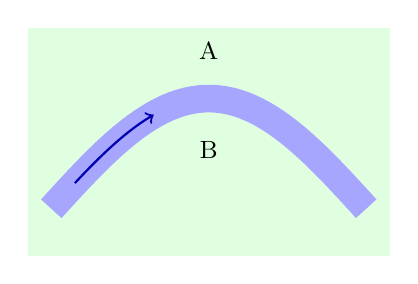
\begin{tikzpicture}[x=1cm, y=1cm, font=\small]
  \fill[green!12] (-0.3,-0.6) rectangle (4.3,2.3);
  \draw[blue!35, line width=10pt] plot[domain=0:4, samples=50]
    (\x,{1.4*sin(\x*45)});
  \draw[blue!70!black, ->, thick] plot[domain=0.3:1.3, samples=20]
    (\x,{1.4*sin(\x*45)});
  \node at (2,2.0) {A};
  \node at (2,0.75) {B};
\end{tikzpicture}
\end{center}
على أي ضفة، A أم B، يبري \omterm{def:g1:landscapes-around-us:water}{النهر} الأرض؟ وعلى أي ضفة
يضع \omterm{def:g3:stones-pebbles-sand:sand}{الرمل}؟
\end{exercise}

\begin{exercise}[$\star$]\label{exo:g5:water-shapes-the-land:6}
في \omterm{def:g1:landscapes-around-us:landform}{الجبال}، يكون قاع \omterm{def:g1:landscapes-around-us:water}{النهر} مغطى بحجارة كبيرة. وقرب \omterm{def:g2:water-on-earth:ocean}{البحر}، يكون مغطى \omterm{def:g3:stones-pebbles-sand:sand}{بالرمل}
\omterm{def:g3:stones-pebbles-sand:sand}{والوحل}. لماذا؟
\end{exercise}

\begin{exercise}[$\star\star$]\label{exo:g5:water-shapes-the-land:7}
طول \omterm{def:g1:landscapes-around-us:water}{نهر} 600 كيلومتر. مجراه الأعلى هو أول
$\frac{1}{6}$ من طوله، ومجراه الأوسط
$\frac{1}{2}$ الذي يليه.
\begin{enumerate}
  \item[(أ)] كم طول المجرى الأعلى؟ وكم طول المجرى الأوسط؟
  \item[(ب)] كم طول المجرى الأدنى؟ وأي كسر من \omterm{def:g1:landscapes-around-us:water}{النهر}
        هو؟
\end{enumerate}
\end{exercise}

\begin{exercise}[$\star\star$]\label{exo:g5:water-shapes-the-land:8}
انظر من جديد إلى صورة \omterm{def:g1:landscapes-around-us:water}{نهر} ماموري كما يُرى من محطة
الفضاء، في الصفحة~\pageref{fig:g5:water-shapes-the-land:mamore}. ما البقع الفاتحة في الجهة الداخلية
للانعطافات؟ وما \omterm{def:g1:landscapes-around-us:water}{البحيرات} الداكنة المقوسة بجانب \omterm{def:g1:landscapes-around-us:water}{النهر}؟ وكيف تكونت؟
\end{exercise}

\begin{exercise}[$\star\star$]\label{exo:g5:water-shapes-the-land:9}
تريد بلدة أن تبني مدرسة جديدة في المروج الخضراء المستوية بجانب
نهرها، لأن الأرض هناك مستوية ورخيصة. ماذا تقول
لمجلس البلدة؟ استعمل كلمتي \emph{\omterm{def:g5:water-shapes-the-land:flood}{فيضان}} و\emph{\omterm{def:g5:water-shapes-the-land:flood}{سهل فيضي}}.
\end{exercise}

\begin{exercise}[$\star\star$]\label{exo:g5:water-shapes-the-land:10}
\omterm{def:g1:landscapes-around-us:water}{أنهار} العالم تحمل إلى \omterm{def:g2:water-on-earth:ocean}{البحر} نحو 12 مليار طن من \omterm{def:g3:stones-pebbles-sand:sand}{الوحل} \omterm{def:g3:stones-pebbles-sand:sand}{والرمل}
كل سنة.
\begin{enumerate}
  \item[(أ)] كم طنًا يساوي ذلك كل شهر، في المتوسط؟
  \item[(ب)] شاحنة كبيرة تحمل 10 أطنان. كم حمولة شاحنة يلزم
        لحمل \omterm{def:g3:stones-pebbles-sand:sand}{وحل} شهر واحد ورمله؟
\end{enumerate}
\end{exercise}

\begin{exercise}[$\star\star\star$]\label{exo:g5:water-shapes-the-land:11}
احكِ قصة حبة \omterm{def:g3:stones-pebbles-sand:sand}{رمل}. تبدأ جزءًا من صخرة عاليًا على
\omterm{def:g1:landscapes-around-us:landform}{جبل}، وتنتهي، بعد سنين كثيرة، في \omterm{def:g5:water-shapes-the-land:delta}{دلتا}. استعمل الكلمات
\emph{\omterm{def:g5:water-shapes-the-land:weathering}{تجوية}} و\emph{\omterm{def:g5:water-shapes-the-land:erosion}{تعرية}} و\emph{\omterm{def:g5:water-shapes-the-land:deposition}{ترسيب}}، وقل ما يحدث
للحبة في المجرى الأعلى والأوسط والأدنى \omterm{def:g1:landscapes-around-us:water}{للنهر}.
\end{exercise}
